\chapter{Кодирование}

\section{Алгоритм Хаффмана (продолжение)}

\begin{tabular}{c c c c c}
 a & b & c & d & e \\
 0.35 & 0.2 & 0.15 & 0.22 & 0.08
\end{tabular}

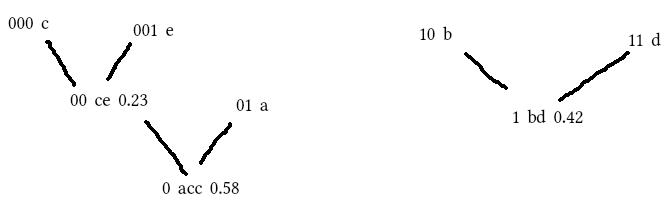
\includegraphics[scale=0.6]{1}


\section{Алгоритм Зива-Лемпеля}

$$\underbrace{a}_1\underbrace{b}_2\underbrace{ab}_3\underbrace{c}_4\underbrace{abc}_5\underbrace{d}_6\underbrace{bc}_7\underbrace{af}_8\underbrace{ac}_9\underbrace{db}_{10}\underbrace{\$}_{11}$$

0a 0b 1b 0c 3c 0d 2c 1f 1c 6b 0\$ \\
записываем [номер известного символа (или комбинации)][новый символ]


\section{Суффиксное дерево }

КАРКАРКАР\$ \\
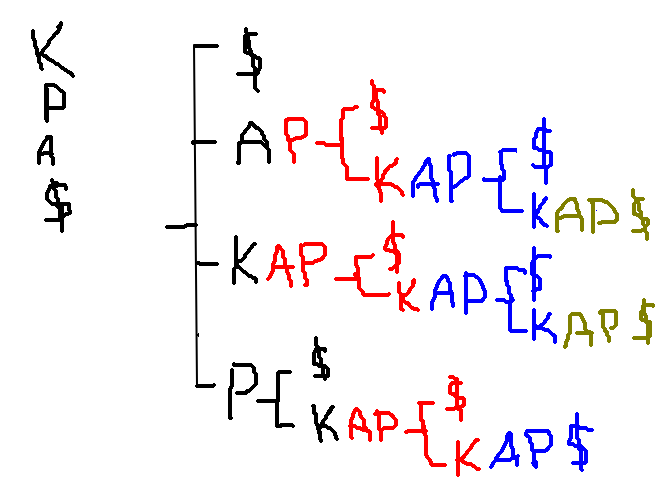
\includegraphics[scale=0.4]{2} \\
очень удобно потом искать подстроку в строке (как ДКА)

\section{Алгоритм Барроуза-Уиллера}

$$ S1 \to S2 \to \begin{cases} S3 \\ \text{Ч}1 \end{cases} $$
При этом по стрелочкам нужно уметь возвращаться

\subsection{Построение строки S2}
Строим суффиксное дерево \\
Для каждого суффикса берём символ, предшествующий ему в строке \\
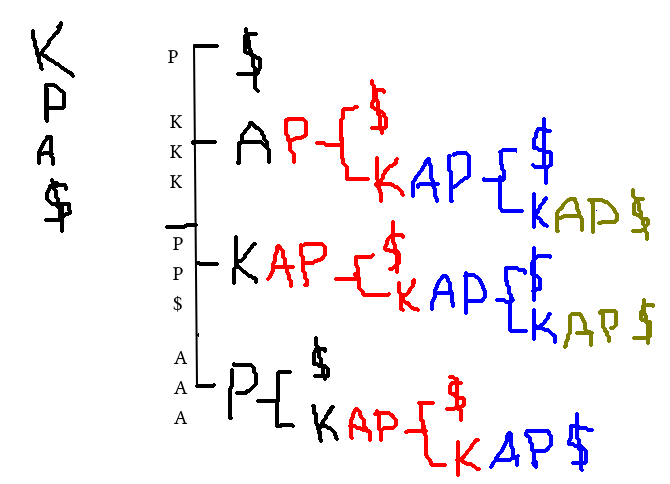
\includegraphics[scale=0.6]{3} \\
РКККРР\$ААА

\subsection{Возврат от S2 к S1}
Записываем символы в лексикографическом порядке \\
Сичтаем количество вхождений в S2, записываем в l[i]: \\
\begin{tabular}{c c c c}
 \$ & А & К & Р \\
 1 & 3 & 3 & 3
\end{tabular} \\ \ \\

a[1] = l[1] \\
a[j] = a[j - 1] + l[j - 1] \\
массив a: \\
\begin{tabular}{c c c c}
 \$ & А & К & Р \\
 1 & 2 & 5 & 8
\end{tabular} \\ \ \\

p[1] = a[символа [1]] \\
a[символа[1]]++ \\
p[j] = a[символа[j]] \\
a[символа[j]]++ \\
массив p: \\
\begin{tabular}{c c c c c c c c c c}
 Р & К & К & К & Р & Р & \$ & А & А & А \\
 8 & 5 & 6 & 7 & 9 & 10 & 1 & 2 & 3 & 4
\end{tabular} \\ \ \\

Строим S1: \\
Записываем \$ в конец, под ним смотрим, куда дальше идти (пока не вернёмся в \$) \\
$ \$\text{РАКРАКРАК (справа налево)} \to \text{КАРКАРКАР}\$ $

\subsection{Построение S3 и Ч1 (алгоритм MoveToFront)}

\begin{tabular}{c | c | c}
    наша строка& Ч1 & temp\\
    \hline
    Р & 0 & Р \\
    К & 0 & КР \\
    К & 1 & КР \\
    К & 1 & КР \\
    Р & 2 & РК \\
    Р & 1 & РК \\
    \$ & 0 & \$РК \\
    А & 0 & А\$РК \\
    А & 1 & \$РК \\
    А & 1 & \$РК \\
\end{tabular} \\
Когда символ ещё не встречался в temp, пишем 0 в Ч1, символ записываем в S3, приписываем символ в начало temp \\
Если встречался, записываем в Ч1 его позицию в temp, переставляем его в начало temp (остальные сдвигаем)\\ \ \\
Получили: \\
S3 = РК\$А \quad Ч1 = 0011210011

\subsection{Возврат от S3 и Ч1 к S2}

\begin{tabular}{c | c | c}
    наша строка& Ч1 & temp\\
    \hline
    Р & 0 & Р \\
    К & 0 & КР \\
    К & 1 & КР \\
    К & 1 & КР \\
    Р & 2 & РК \\
    Р & 1 & РК \\
    \$ & 0 & \$РК \\
    А & 0 & А\$РК \\
    А & 1 & \$РК \\
    А & 1 & \$РК \\
\end{tabular} \\

Если в Ч1 0, берём следующий из S3, приписываем его в начало temp \\
Если в Ч1 не 0, что-то делаем (возможно)
